\section{Introduction}
\label{sec:intro}

The flow past bluff bodies and the formation of vortex structures in their wake has attracted the attention of many scholar over the last decades, as they are ubiquitous in natural environments and in several engineering applications \citep{oertel-1990,williamson-1996b,choi-etal-2008,thompson-etal-2021}. Two-dimensional (2D) and symmetric bluff bodies isolated in free stream are the prototype of this kind of flows.

Most studies on 2D bluff bodies have focused on the circular and square cylinders to characterise the flow bifurcations. The low-$Re$ steady flow generally becomes unstable to oscillatory perturbations that lead to the von K\'{a}rm\'{a}n vortex shedding. The wake past a circular cylinder, for example, undergoes a Hopf bifurcation at a Reynolds number of $Re = U_\infty D /\nu = 47$, where $U_\infty$ is the free stream velocity and $D$ is the radius of the cylinder \citep{noack.eckelmann-1994-globalstability}. This first Hopf bifurcation is generic to flows past isolated 2D bodies that respect the top/down reflectional symmetry \citep{jackson-1987-finiteelementstudy,chiarini-quadrio-auteri-2022b}. The triggering mechanism of this bifurcation is known to result from a global instability \citep{jackson-1987-finiteelementstudy}, which arises when the region of local absolute instability is large enough \citep{chomaz-2005}. Accordingly, \cite{chiarini-quadrio-auteri-2022b} observed that the onset of this instability depends on the size of the wake recirculating region and on the maximum reverse flow velocity.

The secondary instability of the wake past 2D symmetric bluff bodies is generally thought to lead to a three-dimensional (3D) flow. For the circular cylinder, for example, the periodic von K\'{a}rm\'{a}n wake undergoes a secondary pitchfork bifurcation at $Re \approx 190$: the flow becomes 3D but retains the same periodicity. \cite{barkley-henderson-1996} found by Floquet stability analysis that the two-dimensional von K\'{a}rm\'{a}n wake becomes unstable to the synchronous 3D mode $A$ which has spanwise wavelength $\lambda \approx 3.9 D$ at $Re \approx 190$, and to mode $B$ with $\lambda \approx 1.2 D$ at slightly larger $Re$. The long-wavelength Mode A breaks the spanwise translational symmetry of the base flow and gives rise to alternating streamwise vortex loops along the cylinder's span. In contrast, the short-wavelength Mode B preserves mirror symmetry about the mid-span and generates nearly uniform, rib-like vortical structures across the span. The following studies of \cite{henderson-barkley-1996} and \cite{henderson-1997} showed that the onset of modes $A$ and $B$ are due to a supercritical and subcritical bifurcation, respectively. A quasi-periodic mode $S$ with $\lambda \approx 2.5D$ has been also found to become unstable at larger $Re$ \citep{blackburn-lopez-2003,blackburn-etal-2005,blackburn-sheard-2010}. 

\cite{ryan-thompson-hourigan-2005} investigated the secondary instability of the flow past streamlined, elongated cylinders---where no leading-edge (LE) separation occurs---and found that the secondary bifurcation leads to a three-dimensional flow regardless of the body’s aspect ratio. However, they found that the most unstable mode---and consequently, the sequence of bifurcations undergone by the flow---depends sensitively on the aspect ratio, $\AR = L/D$, of the body. They identified mode $A$ and two additional modes, denoted $B'$ and $S'$, by analogy with the canonical modes observed in the wake of a circular cylinder. Mode $B'$ shares the same spatio-temporal symmetry as mode $B$, but its spanwise wavelength and near-wake structure more closely resemble those of mode $S$. Mode $S'$ is characterized by temporal variability from one shedding cycle to the next, similar to mode $S$ observed in the wakes of circular and square cylinders \citep{robichaux-balachandar-vanka-1999}, yet its perturbation field bears a stronger resemblance to mode $B$. \citet{ryan-thompson-hourigan-2005} further reported that for small aspect ratios ($\AR \leq 7.5$), mode $A$ is the first to become unstable, whereas for larger aspect ratios, the initial instability corresponds to mode $B'$.

We now turn to 2D symmetric bluff bodies with sharp LE corners, which are the focus of the present study. In contrast to circular or streamlined cylinders, the presence of sharp LE corners enforces flow separation. A prototypical example of such flows is that past rectangular cylinders with blunt leading edges, which has been extensively studied over the past decades at both moderate \citep{hourigan-thompson-tan-2001,zhang-etal-2023} and high Reynolds numbers \citep{cimarelli-leonforte-angeli-2018,chiarini-quadrio-2021,chiarini-etal-2022,cimarelli-etal-2024}. By varying the aspect ratio $\AR = L/D$, a wide class of body geometries is obtained, ranging from a flat plate normal to the incoming flow as $\AR \to 0$, to a flat plate aligned with the flow as $\AR \to \infty$.
%
Notably, even at intermediate Reynolds numbers ($Re \approx 200$–$400$), beyond the onset of vortex shedding via a primary Hopf bifurcation \citep{chiarini-quadrio-auteri-2021}, the flow exhibits rich and complex dynamics that are strongly dependent on $\AR$ \citep[see, e.g.][]{okajima-1982,nakamura-etal-1991,mills-etal-1995}. For small aspect ratios ($\AR \leq 1$), the shear layers that separate at the LE roll up directly into the wake, forming a classical Bénard--von Kármán vortex street---closely resembling the behaviour observed for circular cylinders. For intermediate aspect ratios ($1 \leq \AR \leq 3$), the separated shear layers intermittently reattach along the lateral surfaces of the cylinder, leading to the formation of intermittent recirculation regions. At larger aspect ratios, the LE shear layers reattach more permanently on the top and bottom surfaces, generating large recirculating bubbles that pulsate periodically.
%
At sufficiently high Reynolds numbers, these high-$\AR$ configurations exhibit vortex shedding from both the LE and trailing-edge (TE) shear layers. The resulting dynamics are governed by the so-called inner leading-edge vortex (ILEV) instability, which leads to frequency locking between the LE and TE shedding. This results in an almost stepwise variation of the Strouhal number, defined as $St_L = fL/U_\infty$, as a function of $\AR$ \citep{okajima-1982,nakamura-etal-1991,hourigan-thompson-tan-2001}; see figure~\ref{fig:StLAR}.
%
\begin{figure}
  \centering
   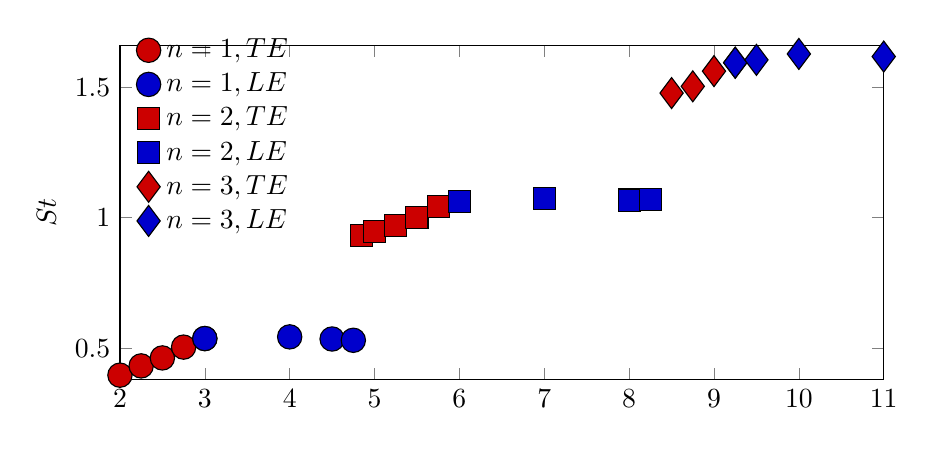
\begin{tikzpicture}



\begin{axis}[%
%width=4.3cm,
%height=3.5cm,
width=0.8\textwidth,
height=0.35\textwidth,
scale only axis,
%grid=both,
%axis lines=middle,
xmin=2,
xmax=11,
ymin=0.38,
ymax=1.66,
%xtick={2, 3, 4, 5, 6, 7, 8, 9, 10, 11},
%ytick={0.4, 0.6, 0.8, 1, 1.2, 1.4, 1.6, 1.8},
%xlabel style={font=\color{white!15!black}},
xlabel={\AR},
ylabel={$St$},
%ymin=0,
%ymax=200,
axis background/.style={fill=white},
legend style={at={(0.01,0.73)}, anchor=west, legend cell align=left, align=left, fill=none, draw=none}
]

\addplot [color=black,only marks,mark=*,mark options={scale=2.2,black,fill=red!80!black}]
  table[row sep=crcr]{%
2       0.396741726829078\\
2.25    0.432248406188668\\
2.5     0.462793383468913\\
2.75    0.504214143890634\\
3       0.536994008053543\\
};
\addlegendentry{$n=1,TE$}

\addplot [color=black,only marks,mark=*,mark options={scale=2.2,black,fill=blue!80!black}]
  table[row sep=crcr]{%
3       0.536994008053543\\
4       0.543439544221324\\
4.5     0.535298051494477\\
4.75    0.530324957725253\\
};
\addlegendentry{$n=1,LE$}


\addplot [color=black,only marks,mark=square*,mark options={scale=2,black,fill=red!80!black}]
  table[row sep=crcr]{%
4.85    0.930407996044941\\
5       0.947349623285183\\
5.25    0.971304878725648\\
5.5     1.000378564453700\\
5.75    1.041747167637721\\
6       1.062464533558995\\
};
\addlegendentry{$n=2,TE$}

\addplot [color=black,only marks,mark=square*,mark options={scale=2,black,fill=blue!80!black}]
  table[row sep=crcr]{%
6       1.062464533558995\\
7       1.073230579537877\\
8       1.067458930414985\\
8.25    1.070000000000000\\
};
\addlegendentry{$n=2,LE$}


\addplot [color=black,only marks,mark=diamond*,mark options={scale=2.8,black,fill=red!80!black}]
  table[row sep=crcr]{%
8.5     1.477258532919061\\
8.75    1.503123920971757\\
9       1.561211928154617\\
9.25    1.593577708455838\\    
};
\addlegendentry{$n=3,TE$}

\addplot [color=black,only marks,mark=diamond*,mark options={scale=2.8,black,fill=blue!80!black}]
  table[row sep=crcr]{%
9.25    1.593577708455838\\    
9.5     1.604355188881951\\
10      1.627228310690177\\
11      1.617135083478177\\
};
\addlegendentry{$n=3,LE$}



%\addplot [color=black,solid,mark=square*,mark options={scale=0.9,black,fill=red!80!black}]
%  table[row sep=crcr]{%
%3       0.609743754434522\\
%4       0.774727821194389\\
%5       0.942866305443131\\
%6       1.100079139112736\\
%7       1.245663824885169\\
%8       1.400191666484032\\
%9       1.546133959599630\\
%10      1.685632118301302\\
%11      1.822225132985195\\
%};



\end{axis}


\end{tikzpicture}%

   \caption{Dependence of $St_L$ on $\AR$ at $Re=400$. Figure adapted from \cite{chiarini-quadrio-auteri-2022}.}
   \label{fig:StLAR}
\end{figure}
%
The stepwise variation of $St_L$ is linked to the number $n$ of LE vortices that can be simultaneously accommodated along the lateral sides of the cylinder---for instance, $n=1$ for $\AR=4$, $n=2$ for $\AR=7$, and $n=3$ for $\AR=9$. \citet{chiarini-quadrio-auteri-2022} identified two distinct shedding regimes, depending on the relative phase between the LE and TE vortices, as well as on which shedding mechanism dominates. When the LE vortices dominate, the shedding frequency locks to the convective passage of LE vortices over the TE, leading to a Strouhal number approximately given by $St \approx n U_c / L$, where $U_c \approx 0.55 U_\infty$ is the mean convection velocity of the LE vortices \citep[see also][]{mills-sheridan-hourigan-2002,tan-thompson-hourigan-2004}. In contrast, when the TE vortices prevail, the shedding frequency resembles that of elongated bodies with the same $\AR$ but with rounded leading edges, where no LE separation occurs.
%
More recently, \citet{zhang-etal-2023} used dynamic mode decomposition at $Re=1000$ to show that the nature of the global feedback mechanism also varies with aspect ratio. For small $\AR$, the feedback loop encompasses the entire separation region and is governed by an impinging shear-layer instability. For larger $\AR$, the loop extends along the full chord of the cylinder and the dynamics are instead dominated by the LE vortex shedding instability.
  
The coexistence of multiple flow regimes and the interactions between LE and TE vortices suggest the presence of distinct secondary instabilities and, consequently, different routes to turbulence. However, to the best of our knowledge, a comprehensive understanding of these secondary instabilities, particularly for flows past elongated rectangular cylinders with aspect ratios $\AR > 1$, remains incomplete.
%
It is well established that the flow past a square cylinder ($\AR=1$) follows a sequence of bifurcations qualitatively similar to that of the circular cylinder, although both the primary and secondary instabilities occur at somewhat lower Reynolds numbers \citep[e.g.][]{jiang-cheng-2018,blackburn-sheard-2010}. Floquet stability analyses by \citet{robichaux-balachandar-vanka-1999}, \citet{blackburn-lopez-2003}, \citet{sheard-fitzgerald-ryan-2009}, and \citet{blackburn-sheard-2010} consistently show that the flow becomes three-dimensional due to mode $A$ at $Re \approx 165$, while modes $B$ and $S$ destabilize only at higher Reynolds numbers. Three-dimensional direct numerical simulations (DNS) by \citet{sheard-fitzgerald-ryan-2009} and \citet{jiang-cheng-an-2018} further investigated the nonlinear saturation of these modes. Notably, \citet{sheard-fitzgerald-ryan-2009} found that both modes $A$ and $B$ arise through supercritical bifurcations, whereas \citet{jiang-cheng-an-2018} argued that mode $A$ instability is subcritical, contrasting with the circular cylinder case \citep{henderson-1997}. They attributed this discrepancy to the limited computational domain used in the former study.
%
The influence of the angle of incidence on the unstable modes was examined by \citet{sheard-fitzgerald-ryan-2009} and \citet{sheard-2011}, who showed that mode $A$ dominates at small and large incidence angles, whereas a subharmonic mode $C$ emerges as the most unstable at intermediate angles. Extending the range of aspect ratios, \citet{choi-yang-2014} studied flows past rectangular cylinders with $\AR \leq 1$, spanning from a flat plate normal to the flow ($\AR \to 0$) to a square cylinder ($\AR=1$). They reported stabilization of modes $A$ and $B$ as $\AR$ decreases, accompanied by the emergence of new synchronous and quasi-periodic modes, denoted $A2$ and $QP2$, respectively \citep[see also][]{thompson-etal-2006}.
%
For the opposite limit, \citet{chaurasia-thompson-2011} and \citet{huang-etal-2017} investigated flows past semi-infinite plates of finite thickness (rectangular cylinders with $\AR \to \infty$). They observed that vortices arising from the LE shear layer due to a Kelvin–Helmholtz instability become unstable to subharmonic three-dimensional perturbations at $Re \approx 380$.
%
Despite these contributions, there remains a significant knowledge gap regarding the secondary bifurcations for rectangular cylinders with intermediate aspect ratios $1 < \AR < \infty$. In a recent study, \citet{chiarini-quadrio-auteri-2022d} focused on the case $\AR=5$ (corresponding to the BARC benchmark \citep{bruno-etal-2014}) within the $n=2$ vortex regime dominated by TE shedding. They identified a secondary instability characterized by a quasi-subharmonic (QS) mode, whose wavemaker \citep{monkewitz-huerre-chomaz-1993} is localized along the longitudinal sides of the cylinder. This instability is driven by the inviscid interaction of vortices generated by the LE shear layer.
%
These findings underscore the need for a systematic characterization of how distinct flow regimes and LE/TE vortex interactions influence the secondary instabilities and transition routes to turbulence in flows past rectangular cylinders with $\AR > 1$.
    
The present work aims to address the existing gap through a comprehensive characterisation of the secondary bifurcation in flows past rectangular cylinders with intermediate aspect ratios. Specifically, we consider cylinders with $1 \leq \AR \leq 9$, combining linear stability analysis and fully nonlinear three-dimensional direct numerical simulations. Our goal is to elucidate how distinct interactions between LE and TE vortices influence the bifurcation scenario, revealing, in particular, the existence of a secondary 2D instability that leads to a deviated wake featuring a non-zero time-averaged lift at intermediate $\AR$. Additionally, new insights into the mechanism underlying mode $A$ are provided; as shown herein, mode $A$ arises exclusively in flow regimes dominated by TE vortices.
%
The remainder of this paper is organized as follows. \S\ref{sec:methods} details the numerical methods and computational setup. The results are presented in sections \S\ref{sec:short}–\S\ref{sec:elongated}. In particular, \S\ref{sec:short} examines the bifurcation scenario for short bodies with $\AR \leq 3$. \S\ref{sec:int} focuses on intermediate aspect ratios $4 \leq \AR < 5$ and reveals the existence of a so far unreported 2D instability leading to a deviated wake in symmetric bluff bodies. Finally, \S\ref{sec:elongated} addresses longer bodies with $\AR \geq 5$, providing new insights into the physics of modes $QS$ and $A$. The paper concludes with a discussion in \S\ref{sec:conc}. Additional details on the influence of $\AR$ on far-wake instabilities are presented in Appendix~\ref{sec:farwake}.
